% DRAFT. Numbers appear ONLY via \input of generated tables (paper/tables/*.tex). Currently PRELIMINARY (v1, single seed).
% Replace with v2 tables:  cp results/v2_tables/*.tex paper/tables/
% No citations are included until the literature table is verified: \cite{TODO} markers must be resolved.
\documentclass[11pt]{article}
\usepackage[margin=1in]{geometry}\usepackage{booktabs,graphicx,amsmath,xcolor,hyperref}
\newcommand{\todo}[1]{\textcolor{red}{[TODO: #1]}}
\title{Does Query-Adaptive Weighting Help? An Empirical Study of Semantic--Chromatic Fusion\\for Colour-Sensitive Product Image Retrieval}
\author{\todo{authors}}\date{}
\begin{document}\maketitle
\begin{abstract}\todo{Write last, after v2 results: problem, setup (frozen CLIP/DINOv2 + HSV histogram, Fashion Product Images small, class-level colour-sensitive relevance), measured findings, conclusion. State honestly that the query-adaptive rule did not materially beat a validation-tuned fixed weight (if v2 confirms).}\end{abstract}

\section{Introduction}
Content-based retrieval with frozen pretrained encoders returns semantically correct but often wrongly coloured items; colour descriptors have the opposite failure \cite{TODO}.
Weighted fusion of the two is standard \cite{TODO}; query-adaptive weighting is a frequently proposed refinement \cite{TODO}.
We ask three questions: (RQ1) how much do semantic and chromatic cues complement each other when relevance requires both category and colour; (RQ2) does a training-free query-adaptive weighting add anything beyond a carefully validated fixed weight; (RQ3) do common pixel-based colour-consistency metrics agree with human colour labels?
\textbf{Contributions} (to be confirmed by v2): \todo{(i) controlled comparison under matched tuning budgets with paired CIs across seeds; (ii) evidence on metric validity (pixel vs.\ human colour); (iii) robustness and cost analysis; (iv) released code.}

\section{Related Work}
\todo{Classical colour/texture descriptors; deep retrieval; hybrid fusion; adaptive/query-dependent weighting; colour-aware re-ranking; evaluation of retrieval robustness. Fill from the verified literature table (paper/LITERATURE\_TABLE.md).}

\section{Problem Formulation}
Let $q$ be a query and $x$ a gallery image. Semantic similarity $S_{sem}(q,x)$ is cosine similarity of frozen embeddings. Chromatic similarity $S_{chr}(q,x)$ is the Bhattacharyya coefficient between $\sqrt{}$-histograms (HSV $16{\times}4{\times}4$ or Lab $4{\times}8{\times}8$) over a central elliptical region.
Both are globally $z$-normalised with statistics from validation pairs only.
\textbf{Relevance.} An image is relevant if it has the same article type \emph{and} the same human-annotated base colour as the query (class-level, not instance-level). Semantic relevance@K is the share of top-$K$ with the query's article type; colour match@K is the share with the query's colour label; we also report a pixel-based consistency (CIEDE2000 between median foreground Lab colours below a threshold $\tau$) as a secondary measure. Because relevance is the conjunction of category and colour label, $\text{Joint}_{\text{label}}@K$ coincides with $P@K$.

\section{Methods Compared}
Fixed fusion $S=\lambda z_{sem}+(1-\lambda)z_{chr}$ with $\lambda$ chosen on validation data (21-point grid).
Adaptive fusion (reference rule): for each query, take the $N$ most semantically similar gallery items; weights $\alpha(q)\propto\lambda_0\sigma_s^{\gamma}$, $\beta(q)\propto(1-\lambda_0)\sigma_c^{\gamma}$ where $\sigma_s,\sigma_c$ are the standard deviations of the normalised scores inside that pool. $\gamma=0$ recovers fixed fusion; the adaptive search grid contains every fixed configuration (search-budget parity). We make no novelty claim for this rule \todo{state after literature check}.
Selection objectives (validation only): mAP (primary) and $P@10$/Joint (secondary, declared after a first exploratory run).

\section{Experimental Setup}
Dataset: Fashion Product Images (small) \cite{TODO}, class filter $\ge$30 images per (article type, colour), random image-level split into validation/test, $S$ seeds. Encoders: CLIP ViT-B/32 and DINOv2-base (frozen). Metrics: mAP, R@1, P@10, semantic relevance@10, colour match@10, Joint, with 95\% bootstrap CIs over queries and paired differences. Robustness: query-side brightness, contrast, saturation, hue shift, blur, occlusion at four fixed severities (gallery unchanged). Cost: CPU brute-force scoring latency and per-image storage.
\todo{Hardware, software versions, seeds, licence statement for dataset.}

\section{Results}
\subsection{Complementarity of semantic and chromatic cues (RQ1)}
\begin{table}[t]\centering\small
\caption{Main comparison on the test split (mean$\pm$SD over seeds where more than one run exists).}\label{tab:main}
\resizebox{\linewidth}{!}{\begin{tabular}{llrrrrrrr}\toprule
encoder & method & mAP & R@1 & P@10 & Sem@10 & ColLab@10 & JointLab@10 & Col@10 \\ \midrule
openai\_clip-vit-base-patch32 & Colour only (HSV) & 0.113 & 0.394 & 0.280 & 0.413 & 0.618 & 0.280 & 0.979 \\
openai\_clip-vit-base-patch32 & Semantic only & 0.291 & 0.552 & 0.447 & 0.850 & 0.530 & 0.447 & 0.889 \\
openai\_clip-vit-base-patch32 & Fixed, $\lambda$=0.5 & 0.305 & 0.638 & 0.520 & 0.801 & 0.640 & 0.520 & 0.965 \\
openai\_clip-vit-base-patch32 & Fixed, val-best (mAP) & 0.320 & 0.622 & 0.514 & 0.841 & 0.605 & 0.514 & 0.940 \\
openai\_clip-vit-base-patch32 & Adaptive, val-best (mAP) & 0.321 & 0.627 & 0.518 & 0.838 & 0.612 & 0.518 & 0.944 \\
openai\_clip-vit-base-patch32 & Fixed, val-best (mAP), Lab hist. & 0.321 & 0.598 & 0.508 & 0.844 & 0.598 & 0.508 & 0.950 \\
facebook\_dinov2-base & Colour only (HSV) & 0.113 & 0.394 & 0.280 & 0.413 & 0.618 & 0.280 & 0.979 \\
facebook\_dinov2-base & Semantic only & 0.258 & 0.405 & 0.361 & 0.873 & 0.423 & 0.361 & 0.846 \\
facebook\_dinov2-base & Fixed, $\lambda$=0.5 & 0.318 & 0.619 & 0.523 & 0.838 & 0.624 & 0.523 & 0.961 \\
facebook\_dinov2-base & Fixed, val-best (mAP) & 0.320 & 0.613 & 0.512 & 0.851 & 0.600 & 0.512 & 0.951 \\
facebook\_dinov2-base & Adaptive, val-best (mAP) & 0.319 & 0.617 & 0.518 & 0.848 & 0.611 & 0.518 & 0.954 \\
facebook\_dinov2-base & Fixed, val-best (mAP), Lab hist. & 0.320 & 0.568 & 0.496 & 0.858 & 0.579 & 0.496 & 0.968 \\
\bottomrule\end{tabular}}
\end{table}
\todo{After v2: describe fusion vs.\ single-modality results with CIs. In the preliminary single-seed run (v1), fusion improved human-label colour match and Joint over semantic-only for both encoders at a small cost in category relevance; re-verify.}
\begin{figure}[t]\centering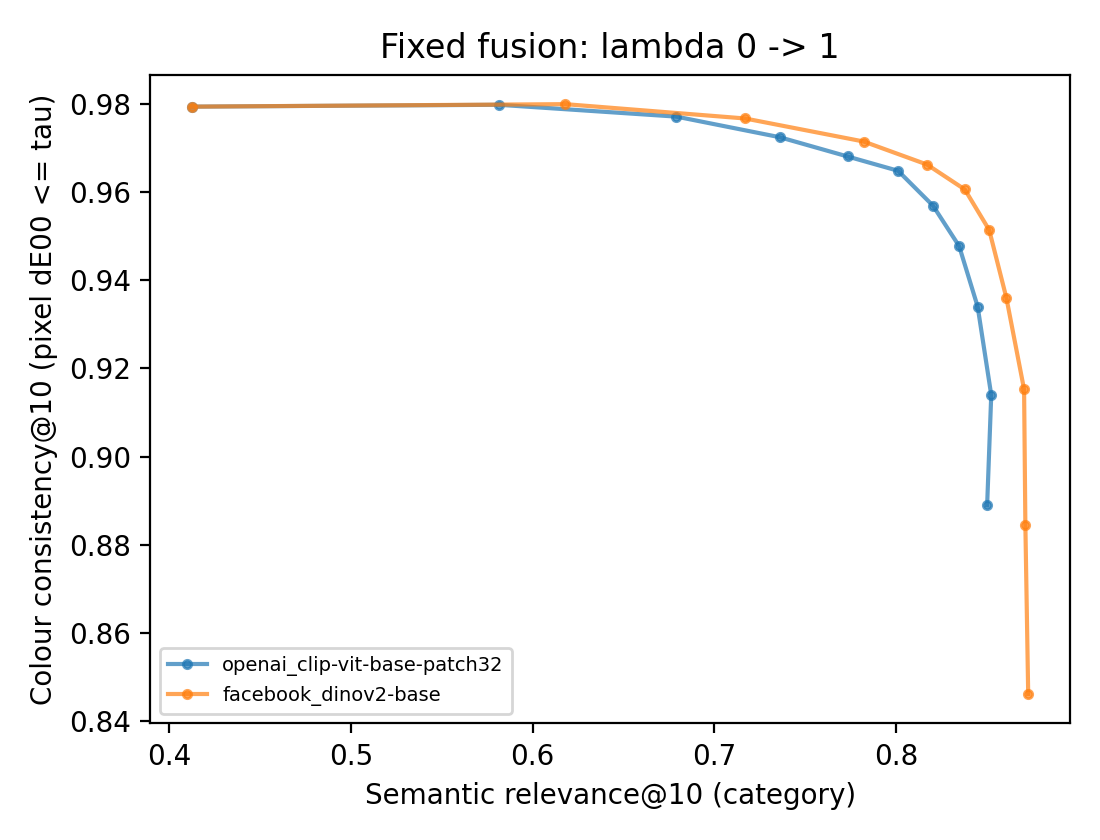
\includegraphics[width=.6\linewidth]{figures/fig4_tradeoff.png}\caption{Semantic--colour trade-off under fixed fusion ($\lambda$ swept; reported, not tuned).}\end{figure}

\subsection{Does query-adaptive weighting help? (RQ2)}
\begin{table}[t]\centering\small
\caption{Adaptive minus fixed-weight fusion (paired over test queries; last column = seeds whose 95\% bootstrap CI excludes 0). Seven metrics, no multiplicity correction.}\label{tab:paired}
\resizebox{\linewidth}{!}{\begin{tabular}{llrrr}\toprule
encoder & comparison & metric & mean\_diff & seeds\_CI\_excl\_0 \\ \midrule
openai\_clip-vit-base-patch32 & adaptive\_minus\_best\_fixed & AP & +0.0014 & 1/1 \\
openai\_clip-vit-base-patch32 & adaptive\_minus\_best\_fixed & R@1 & +0.0056 & 0/1 \\
openai\_clip-vit-base-patch32 & adaptive\_minus\_best\_fixed & Sem@10 & -0.0028 & 1/1 \\
openai\_clip-vit-base-patch32 & adaptive\_minus\_best\_fixed & Col@10 & +0.0035 & 1/1 \\
openai\_clip-vit-base-patch32 & adaptive\_minus\_best\_fixed & Joint@10 & +0.0006 & 0/1 \\
openai\_clip-vit-base-patch32 & adaptive\_minus\_best\_fixed & ColLab@10 & +0.0066 & 1/1 \\
openai\_clip-vit-base-patch32 & adaptive\_minus\_best\_fixed & JointLab@10 & +0.0045 & 1/1 \\
openai\_clip-vit-base-patch32 & adaptive\_minus\_fixed\_lambda0.5 & AP & +0.0161 & 1/1 \\
openai\_clip-vit-base-patch32 & adaptive\_minus\_fixed\_lambda0.5 & R@1 & -0.0113 & 0/1 \\
openai\_clip-vit-base-patch32 & adaptive\_minus\_fixed\_lambda0.5 & Sem@10 & +0.0366 & 1/1 \\
openai\_clip-vit-base-patch32 & adaptive\_minus\_fixed\_lambda0.5 & Col@10 & -0.0213 & 1/1 \\
openai\_clip-vit-base-patch32 & adaptive\_minus\_fixed\_lambda0.5 & Joint@10 & +0.0172 & 1/1 \\
openai\_clip-vit-base-patch32 & adaptive\_minus\_fixed\_lambda0.5 & ColLab@10 & -0.0280 & 1/1 \\
openai\_clip-vit-base-patch32 & adaptive\_minus\_fixed\_lambda0.5 & JointLab@10 & -0.0021 & 0/1 \\
facebook\_dinov2-base & adaptive\_minus\_best\_fixed & AP & -0.0018 & 0/1 \\
facebook\_dinov2-base & adaptive\_minus\_best\_fixed & R@1 & +0.0042 & 0/1 \\
facebook\_dinov2-base & adaptive\_minus\_best\_fixed & Sem@10 & -0.0035 & 1/1 \\
facebook\_dinov2-base & adaptive\_minus\_best\_fixed & Col@10 & +0.0023 & 0/1 \\
facebook\_dinov2-base & adaptive\_minus\_best\_fixed & Joint@10 & -0.0016 & 0/1 \\
facebook\_dinov2-base & adaptive\_minus\_best\_fixed & ColLab@10 & +0.0105 & 1/1 \\
facebook\_dinov2-base & adaptive\_minus\_best\_fixed & JointLab@10 & +0.0059 & 1/1 \\
facebook\_dinov2-base & adaptive\_minus\_fixed\_lambda0.5 & AP & +0.0002 & 0/1 \\
facebook\_dinov2-base & adaptive\_minus\_fixed\_lambda0.5 & R@1 & -0.0014 & 0/1 \\
facebook\_dinov2-base & adaptive\_minus\_fixed\_lambda0.5 & Sem@10 & +0.0099 & 1/1 \\
facebook\_dinov2-base & adaptive\_minus\_fixed\_lambda0.5 & Col@10 & -0.0069 & 1/1 \\
facebook\_dinov2-base & adaptive\_minus\_fixed\_lambda0.5 & Joint@10 & +0.0035 & 0/1 \\
facebook\_dinov2-base & adaptive\_minus\_fixed\_lambda0.5 & ColLab@10 & -0.0131 & 1/1 \\
facebook\_dinov2-base & adaptive\_minus\_fixed\_lambda0.5 & JointLab@10 & -0.0051 & 1/1 \\
\bottomrule\end{tabular}}
\end{table}
\todo{After v2: report equivalence against the pre-declared margin ($\pm0.01$ on mAP and Joint$_{label}$@10); in v1 differences were about one point or less with inconsistent sign across encoders, and the adaptive rule traded colour match for category relevance relative to $\lambda=0.5$.}

\subsection{Is pixel colour similarity a valid proxy for human colour? (RQ3)}
\todo{Table: ROC-AUC of HSV/Lab Bhattacharyya, CIEDE2000 on foreground median colour, and semantic cosine for predicting colour-label agreement (paper/tables/table\_metric\_agreement.tex from v2). Also the $\tau$ sensitivity table; v1 showed the 90th-percentile threshold (29.7 $\Delta E_{00}$) makes the pixel metric nearly saturated.}

\subsection{Where does colour fusion help? Robustness and cost}
\todo{Per-colour/achromatic-vs-chromatic breakdown (table\_colour\_group), robustness figure/table, latency and storage table, qualitative examples and failure cases from per\_query.csv.}

\section{Limitations and Ethical Considerations}
Class-level rather than instance-level relevance; low-resolution images; coarse and noisy colour labels; single dataset; frozen encoders only; results depend on the validation objective used to choose $\lambda$; several analyses were added after a first exploratory run (see protocol log). No external validation yet \todo{Stanford Online Products or another dataset}. Dataset licence and redistribution terms \todo{verify}.

\section{Conclusion}\todo{After v2.}
\bibliographystyle{plain}\bibliography{references}
\end{document}
